\chapter{Objectives}

\begin{itemize}
    \item Certify data quality in lumisection granularity
    \begin{itemize}
        \item Classification on the basis of actual data distributions per LS
    \end{itemize}
    \item Reduce manual work of DC Experts
\end{itemize}

\section{Expectation}
The most important aim of this work is to reduce the offline shifter work where we should provide the tools to reduce their work if some data are totally bad or perfectly good and let them inspect only for a few grey zones.
In order to separate a kind of data quality, we have to define some decision values from some mathematical models to determine the data quality by finding some threshold to separate them.
For the ideal case, we might see the good lumisection that looks perfectly good, bad lumisection that looks terribly skew and the grey zone where some of those two kinds of lumisection are overlapping.

\begin{figure}[h!]
    \centering
    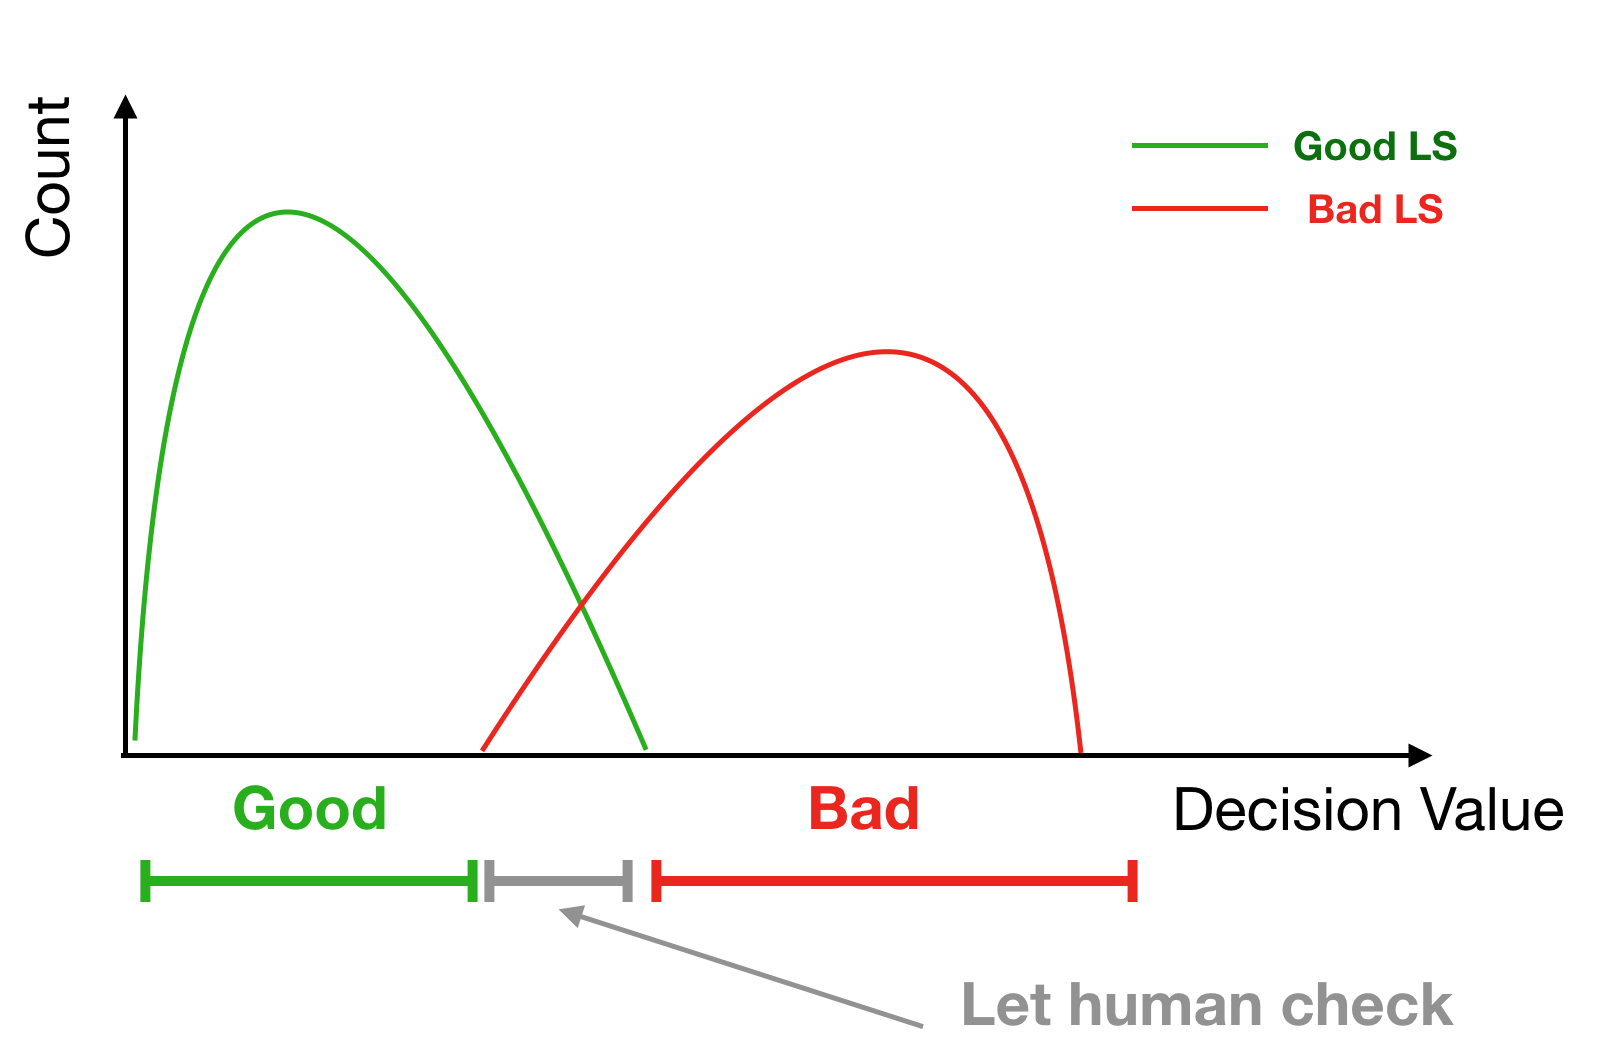
\includegraphics[width=0.7\textwidth]{images/expected_greyzone.png}
    \caption{Three possible regions of prediction}
    \label{fig:expected_greyzone}
\end{figure}

\section{Proposal For an Alternative Approach}
Again, the purpose of this work is not to redefine the certification process but mimic a shifter and reduce their work if there is an obvious case.
Then the automatic DCS bit flagging will stay but we apply the algorithm on top of it rather than remove the criteria.
The quantity value of each data point are physical quantities such as
\begin{enumerate}
    \item \textbf{Features} transverse momentum, azimuth angle from the beamline, etc.
    \item \textbf{Objects} Mapped to the relevant promary dataset (i.e. trakcs to ZeroBias, muons to SingleMuon and so on)
\end{enumerate}
Since each run contain a lot of lumisection which probably too much for processing the certification, \cite{fiori_ml_dc_florence} offers a way to certify data by run and lumisection levels where there is a supervised learning apply in the whole run and feeding only the grey zone to inspect by lumisection to investigate the outlier on step 2 as in the Figure \ref{fig:cartoon}.
\begin{figure}[h!]
    \centering
    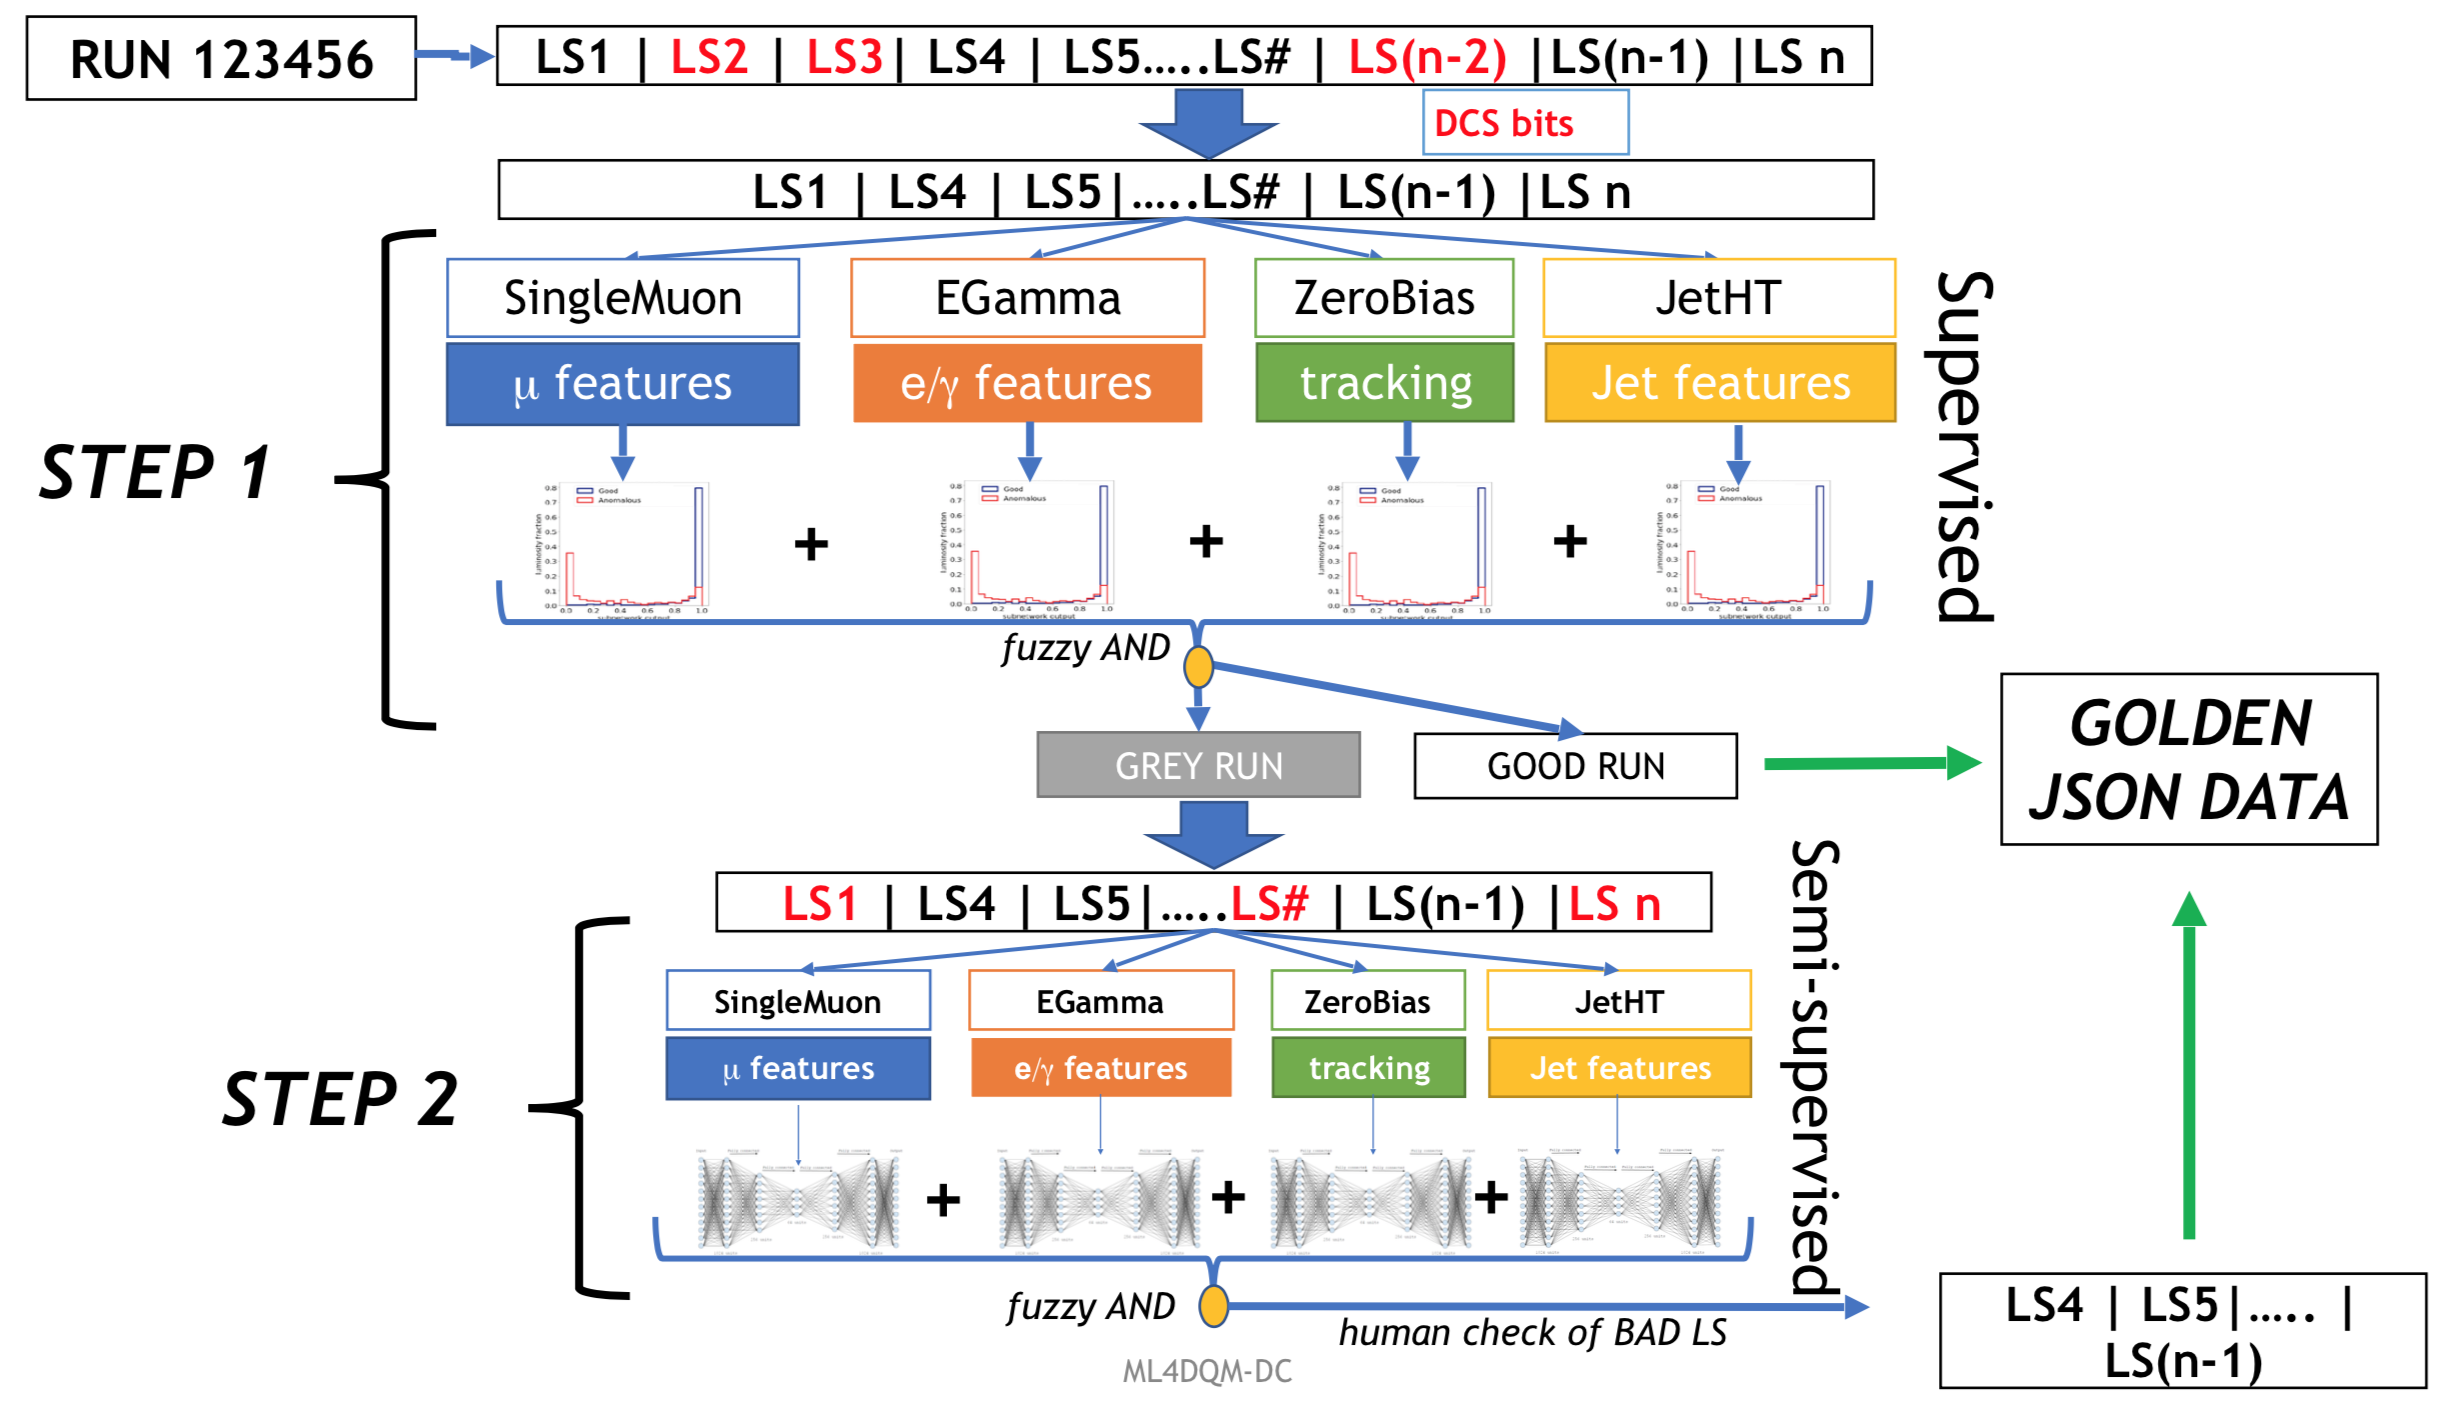
\includegraphics[width=\textwidth]{images/cartoon.png}
    \caption{ML certification procedure, image taken from \cite{fiori_ml_dc_florence}}
    \label{fig:cartoon}
\end{figure}